\subsection{Change}
\label{sec:Suggestion:Change}

\begin{figure}[t]
    \centering
    
\includegraphics[width=\columnwidth]{images/Suggestion.pdf}
    \caption{A \textsf{Suggestion} holds for a single \textsf{Change} linked to 
		elements in a View Type through \textsf{Relation}s, and consists of a set of \textsf{Recommendation}s.}
    \label{fig:Suggestion}
\end{figure}

A \textsf{Change} refers to an \textsf{Operator} that may be parameterised with 
extra data, and contains contextual information (in \textsf{ApplicationPattern}\LC{what is meant by this? ApplicationPattern is not visible in any Figure, and Googling it, is not immediately clear which if any specific design pattern it refers to, if that's what's intended}). 
Change \textsf{Operator}s may target \emph{any} instantiable \metamodel element, 
thus referring to the class \textsf{NamedElement} in \textsc{Mof}. Note that we 
will distinguish between \emph{primitive} and \emph{complex} \textsf{Operator}s,
depending on the number of such \metamodel elements an \textsf{Operator} acts on.

Since \viewtypes are structurally \metamodels, we reviewed the literature to
identify relevant change \textsf{Operator}s. In our work, we integrate all 27 \textit{primitive} and seven of the 34 \textit{complex} operators in the change catalogue proposed by Herrmannsdoerfer et al.~\cite{herrmannsdoerfer_extensive_2011}.
These seven were selected because they constitute 72\% of all complex changes appearing in a large case study (cf. \cite{khelladi_detecting_2015}). 

\textsf{Operator}s are enriched with a \emph{severity}: \emph{Major}
(abbreviated as \textsf{M}), \emph{miNor} (\textsf{N}) and \emph{Ignore} 
(\textsf{I}). 
When applied to a \metamodel, the \textsf{Operator}s in \textsf{I} have no effect
on the corresponding \viewtypes; \textsf{Operator}s that can break the relationship
between \textsf{MM }and its \viewtypes are categorised as \textsf{M}; the rest of the
\textsf{Operator}s are \textsf{N}, since they are not breaking and can enrich 
the \viewtypes with additional information.\LC{Idea I've applied to table, to save space/cognitive load on table: dropped the 'I' operator rows from the table completely; instead adding next sentence here:} The seven \textsf{Operator}s \textsf{Make/Drop Class Abstract}, \textsf{Make/Drop Attribute Identifier}, \textsf{Make/Switch Reference Composite}, and \textsf{Pull Property} are of type \textsf{I} and hence not included in Table~\ref{tab:suggestions} of suggestions per change operator.

\begin{figure}[t]
    \centering
    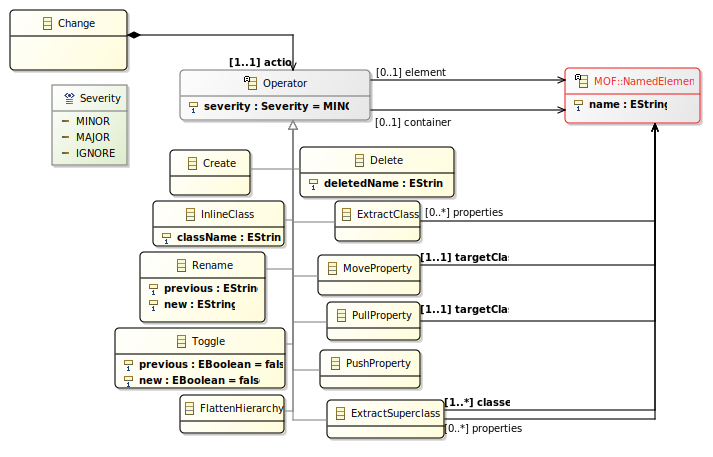
\includegraphics[width=\columnwidth]{Change.pdf}
    \caption{Possible \textsf{Operator}s for \metamodel evolution.}
    \label{fig:Change}
\end{figure}

The evolution steps of Figure \ref{fig:FSM} make use of different \textsf{Operator}s.
\begin{itemize}
	\item In Step 1 (depicted from Figure \ref{fig:FSM:Init} to \ref{fig:FSM:Relevant}),
	the following sequence of \textsf{Operator}s is applied:
	$$\langle \mathsf{PushProperty} \cdot \mathsf{Rename} \cdot \mathsf{Rename} \rangle$$
	First, \textsf{PushProperty} pushes down $\mathsf{Named} \squaredots \mathsf{name}$
	(i.e. pushes down the \textsf{element} \textsf{name} in the \textsf{container}
	\textsf{Named})
	into each subclass (namely, \textsf{FSM}, \textsf{State} and \textsf{Transition});
	then \textsf{Rename} is applied to the \textsf{element} \textsf{name}, 
	located respectively in \textsf{container}s $\mathsf{FSM}$ and 
	$\mathsf{Transition}$, thus obtaining the result of Figure \ref{fig:FSM:Relevant}.
	
	\item Step 2 only consists of the following \textsf{Operator} sequence:
	$$\langle \mathsf{Create} \cdot \mathsf{Create} \cdot \mathsf{Create} \rangle$$
	where each \textsf{Operator} adds a new Attribute \textsf{element} in 
	\textsf{container} \textsf{Transition}, ending up in the situation of
	Figure \ref{fig:FSM:Guard}.
	
	\item Step 3 requires a longer sequence of \textsf{Operator}s, since it creates
	a new class hieararchy under \textsf{Expression}. However, this sequence may
	start with the following:
	$$\langle \mathsf{Delete}^3 \cdot \mathsf{Create}^2 \cdot \ldots \rangle$$
	The initial \textsf{Delete}s undo the \textsf{Create} operations of Step 2
	(thus, referring to the same \textsf{element}s and \textsf{container}); and
	the two following \textsf{Create}s create the new \textsf{Expression} class
	(with the default package as a \textsf{container}) and the \textsf{guard}
	reference (with \textsf{Transition} as a \textsf{container}).
\end{itemize}
With these examples, we immediately notice that some \textsf{Operator}s
in a \textsf{Change} sequence may depend on previous ones (e.g. \textsf{Rename}
in Step 1 should only be performed after \textsf{PushProperty}); while others
may freely commute (e.g. the \textsf{Create} in Step 2 may be performed in any 
order).